\documentclass[11pt]{amsart}
\usepackage{amssymb,amsmath,amsthm,newlfont,enumerate, standalone}
\usepackage{tikz-cd}
\usepackage{pgfplots}
\pgfplotsset{compat=1.18}
\usepgfplotslibrary{fillbetween}
\usetikzlibrary{intersections}
\usetikzlibrary{patterns}

\begin{document}

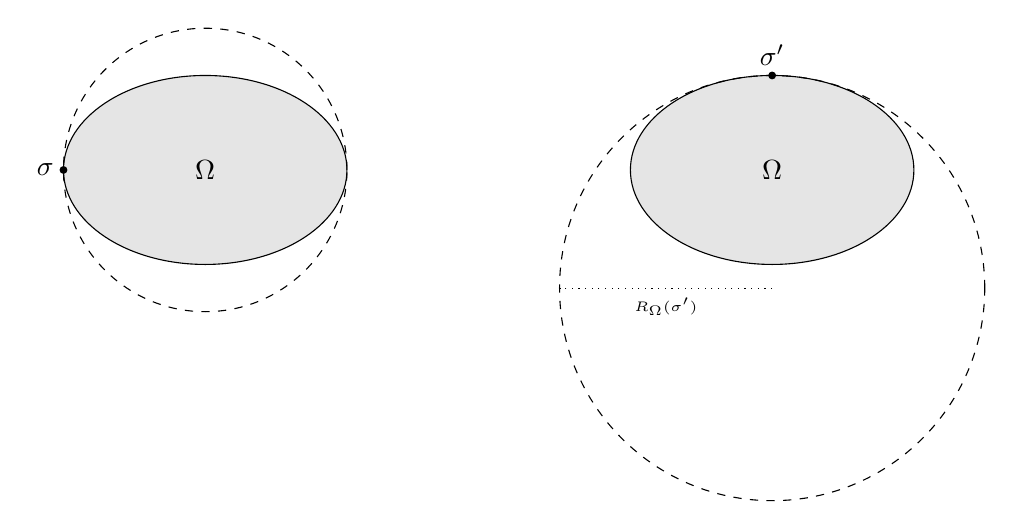
\begin{tikzpicture}[scale=0.6]
\fill[fill=gray!20] (-6,0) ellipse (3 and 2);
\draw (-6,0) node{$\Omega$};
\draw (-6,0) ellipse (3 and 2);
\draw[dashed] (-6,0) circle(3);
\filldraw (-9,0) circle (2pt) node[left]{$\sigma$};
\fill[fill=gray!20] (6,0) ellipse (3 and 2);
\draw (6,0) node{$\Omega$};
\draw (6,0) ellipse (3 and 2);
\draw[dashed] (6,-5/2) circle(9/2);
\filldraw (6,2) circle (2pt) node[above]{$\sigma'$};
\draw[ dotted] (6, -5/2) -- (3/2, -5/2) node[midway, below]{\tiny $R_\Omega(\sigma')$};
\end{tikzpicture}

\end{document}